\documentclass[12pt,a4paper]{book}
\usepackage[utf8]{inputenc}
\usepackage[spanish]{babel}
\usepackage{amsmath}
\usepackage{amsfonts}
\usepackage{amssymb}
\usepackage{makeidx}
\usepackage{graphicx}
\usepackage{hyperref}
\usepackage{setspace}
\usepackage{epigraph}
\usepackage{booktabs}
\usepackage[T1]{fontenc}
\usepackage{times}
\usepackage{lipsum}
\renewcommand{\baselinestretch}{2}
\renewcommand{\tablename}{Tabla}
\AtBeginDocument{\renewcommand\tablename{Tabla}}
\usepackage[left=3cm,right=2.5cm,top=3cm,bottom=3cm]{geometry}
\hypersetup{colorlinks,linkcolor={blue},citecolor={blue},urlcolor={red}} 
\title{Calibración de un Prototipo de Detector Cherenkov analizando el Decaimiento del Muón}
\date{Mayo 2021}
\author{Quispe Calloapaza, David Saúl y Quispe Mamani, Sonia Diana}

\begin{document}
	\begin{titlepage}
	\begin{center}
		{\Large \textbf{Universidad Nacional de San Agustín de Arequipa}}\\
		{\Large \textbf{Facultad de Ciencias Naturales y Formales}}\\
		\vspace{1mm}
		{\Large \textbf{Escuela profesional de Física}}\\
		\begin{figure}[h]
			\centering
			
\includegraphics[scale=0.3]{FIGURAS/Logo_unsa.png}
		\end{figure}
		\vspace{1mm}
		\rule{\linewidth}{0.75mm}\\
		\vspace{1mm}
		\begin{spacing}{1.5}
			{\LARGE \textbf{Monitoreo de la estabilidad de respuesta de un prototipo de detector Cherenkov analizando el decaimiento del Muón}}
		\end{spacing}
		\rule{\linewidth}{0.75mm}\\
	\end{center}

    \begin{spacing}{1}
    	\epigraph{Tesis presentada por:\\
    	Quispe Calloapaza, David Saúl\\
    	Quispe Mamani, Sonia Diana\\
    	\vspace{3mm}
    	Para optar el grado de:\\ Bachiller en Física\\
    	\vspace{3mm}
    	Asesores:\\
    	Mg. Rolando Moisés Perca Gonzáles\\
    	Msc. Luis Otiniano Ormachea\\
    	Dr. José Bellido Cáceres}{}
	
	\begin{center}
		Arequipa - Perú\\
		2021
	\end{center}
	\end{spacing}
\end{titlepage}
	
	\tableofcontents
	
	\listoffigures
	
	\chapter{Introducción}
Con la llegada, en 1906, del telescopio óptico de Galileo, se obtuvo el primer avance en las observaciones del universo, que en ese contexto se podían hacer únicamente empleando los ojos de manera directa. Se expandió por primera vez el universo observable para el hombre. Más adelante, nos dimos cuenta que el telescopio era un instrumento limitado para observar el universo, debido a que unicamente podiamos observar la región visible del espectro electromagnético \cite{Vazquez}. Más adelante se emplearían métodos novedosos para observar regiones, del espectro electromagnético, fuera del visible.  

El físico austriaco Víctor Hess entre los años 1911-1912 realizó experimentos cruciales, los cuales ponían en manifiesto la existencia de una radiación cuyo origen era del espacio exterior. Hess publicó los resultados de sus experimentos concluyendo lo siguiente: "Los resultados de estas observaciones parecen poder interpretarse admitiendo sencillamente que una radiación con gran poder de penetración procede de la parte superior de la atmósfera y, aunque progresivamente atenuada por ésta, produce, incluso en las zonas más bajas, una parte de la ionización observada en las cámaras cerradas. La intensidad de está radiación parece estar afectada por pequeñas variaciones aleatorias" \cite{Lugo}.

Hoy en día, se emplean distintos tipos de detectores para poder observar el universo en un rango más amplio de energía, todo esto con el fin de saber lo que hay y como ha ido evolucionando nuestro universo. Los rayos gamma de alta energía, por ejemplo, son producidos en fenómenos llamados GRB (destello de rayos gamma por sus siglas en inglés Gamma Ray Burst) que toman lugar en fenómenos muy violentos en universo como colisión de estrellas masivas, nucleos activos de galaxia, explosiones de estrellas tipo supernova, etc \cite{PEREZY2009}. Por lo que la detección de esta radiación proveniente del espacio exterior nos brinda aún más conocimiento sobre lo sucede en el universo y la evolución de este.
	
	\chapter{Rayos Cósmicos}\label{RAYOS_COSMICOS}
Uno de los rangos de interés para la astrofísica son los rayos cósmicos (CR's por sus siglas en inglés Cosmic Rays) de alta energía. Los CR's consisten en su mayoría de núcleos atómicos ionizados, además de electrones, positrones, antiprotones, rayos gamma y neutrinos que van llegando a la Tierra de algún lugar en el universo, también se les conoce como CRs primarios. Estos CR's se extienden desde poco menos de $1$GeV hasta más allá de los $100$EeV. Con el objetivo de observarlos se han empleado diferentes técnicas de detección dependiendo del rango de energía en estudio.

Por ejemplo, por debajo de pocos cientos de TeV, lo CR's tienen un flujo muy grande de $5\times 10^6$m$^{-2}$sr$^{-1}$yr$^{-1}$, y pueden ser detectado de manera directa por satelites antes de que estos interaccionen con la atmósfera. Pero para CRs con pocos cientos por encima de los TeV el flujo de estos llegan a un valor menor de $50$m$^{-2}$sr$^{-1}$yr$^{-1}$ \cite{MOLLERACH201885}, donde la detección directa ya no es práctica , pues se tendría que tener satélites capaces de abarcar grandes áreas, por lo que se recurren a métodos de detección indirectos que se explicará más adelante. Entonces, la construcción de estaciones de capaces de detectar rayos cósmicos en distintas partes del mundo, brindan información para ampliar el conocimiento del universo observable en astrofísica.

\begin{figure}
	\centering
	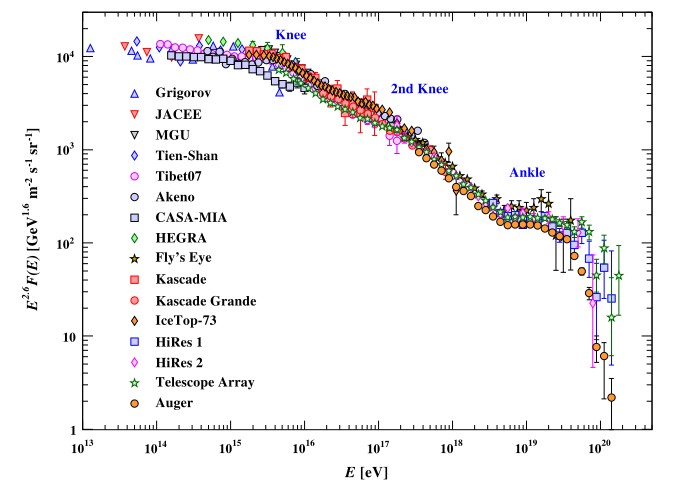
\includegraphics[scale = 0.5]{FIGURAS/ESPECTRO_RC.png}
	\caption{Espectro de flujo de rayos cósmicos a altas energías, multiplicado por $E^{2.6}$ para una mejor observación, en función de la energía \cite{MOLLERACH201885}.}
	\label{Espectro_CR}
\end{figure}

La figura \ref{Espectro_CR}, nos muestra el espectro de flujo de CR's a altas energías, este espectro sigue una ley de potencias de aproximadamente $d\phi /dE \propto E^{-\gamma}$ con un valor de $\gamma \simeq 3$, este espectro muestra algunas interesantes características.
\begin{itemize}
	\item Por encima de pocos cientos de GeV hasta pocos cientos de PeV, el espectro muestra un valor de $\gamma \simeq 2.7$.
	\item En la zona conocida como primera rodilla o ``kne" ($\sim 4 \mbox{PeV}$) el espectro cambia a $\gamma \simeq 3$.
	\item En la zona conocida como segunda rodilla o ``seoncd knee" ($\sim 0.1 \mbox{EeV}$) el espectro cambia a $\gamma \simeq 3.3$.
	\item En la zona concida como tobillo o ``ankle" ($\sim 5 \mbox{EeV}$), el espectro cambia nuevamente con $\gamma \simeq 2.6$.
\end{itemize}

Note que el flujo determinado por varios experimentos varía debido a las técnicas de detección y calibración de energía usado en los distintos experimentos. Además de que, para la detección de CR de altas energías se estudian las cascadas atomosféricas formadas por estos, ver sec. \ref{EAS}.
	
	\chapter{Cascadas atmosféricas y efecto Cherenkov} \label{EAS_Y_CHERENKOV}
\section{Cascadas atmosféricas} \label{EAS}
	Las cascadas atmosféricas (o EAS por sus siglas en inglés Extensive Air Shower) tienen su origen gracias a la interacción de un CR primario, que llega a la Tierra, con la atmósfera terrestre. La mayor parte de estas EAS son iniciadas por CR con energías mayores a $10^{13}$ eV o $10$ TeV. Cuando estos procesos de colisión son dominados por hadrones se forma lo que conoce como cascada hadrónica, que se propaga en la dirección del momento inicial de la partícula primaria. Luego, muones y neutrinos se forman a partir del decaimiento de piones cargados y kaones, formandose también lo que se conoce como cascada muónica.

	\begin{figure}[h]
		\centering
		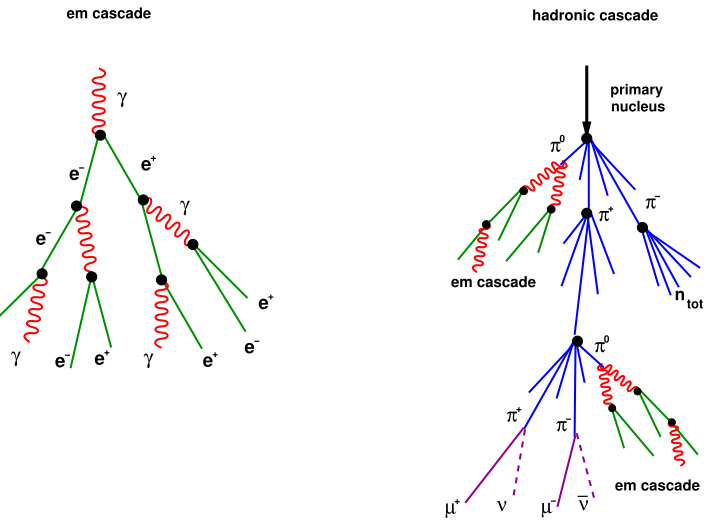
\includegraphics[scale = 0.5]{FIGURAS/CASCADA_LONGITUDINAL.png}
		\caption{Desarrollo longitudinal de una casacada puramente electromagnética y una cascada hadrónica. Los puntos negros representan el lugar de la interacción de la partícula con un núcleo de la atmósfera \cite{MOLLERACH201885}.}
		\label{Cascada_longitudinal}
	\end{figure}

	Los piones neutros y otras partículas decaen en electrones y rayos gamma, formándose así la cascada electromagnética. Aquí se involucran procesos como creación de pares y Bremsstrahlung. De esta manera, una partícula primaria con alta energía puede generar una cascada con gran cantidad de partículas y fotones \cite{GRIEDER2010}.  Dichas cascadas se propagan esencialmente a la velocidad de la luz y pueden alcanzar la superficie terrestre si el CR primario es suficientemenete energético.

	Las cascadas pueden ser iniciadas por hadrones, fotones y electrones, las cascadas iniciadas por fotones o electrones se les conoce como cascadas puramente electromagnéticas. Los fotones de alta energía energía interaccionan con los núcleos de la atmósfera generando la creación de pares $e^+$ y $e^-$, los electrones y positrones interaccionan con los núclos de la atmósfera para porducir fotones mediante Bremsstrahlung \cite{MOLLERACH201885}. A este desarrollo de las cascadas a lo largo de la profundidad atmosférica (medida en gm/cm$^2$) se le conoce como desarrollo longitudinal, la figura \ref{Cascada_longitudinal} nos muestra el desarrollo longitudinal de una cascada puramente electromagnética (inciada por un fotón) y una cascada hadrónica.

\section{Efecto Cherenkov} \label{EFECTO_CHERENKOV}

	
	\chapter{Técnicas de detección}\label{TECNICAS_DE_DETECCION}
El hombre ha realizado diversos experimentos científicos de aceleradores de partículas, como el Gran Colisionador de Hadrones o LHC (Large Hadron Collider) ésto con la finalidad de acelarar las partículas para que colisionen entre sí y generar subproductos que, al estudiarlos, nos dan un idea más clara del mundo subatómico, sin embargo, sólo puede llegar a energías limitadas, alrededor de los TeV. Es por ello que radica la importancia del estudio de astropartículas, su origen galáctico y como estos se relacionan a eventos de gran magnitud, como remanentes de supernovas, núcleos activos de galaxias, agujeros negros entre otros. Estos eventos son considerados fuentes naturales de aceleadores de partículas y llegan a energías desde los TeV hasta los EeV \cite{Gonzales}. En contra parte, los rayos cósmicos y los rayos gamma son muy difíciles de detectar debido a sus interacción con moléculas de la atmósfera, debido a ésto se utilizan diversas técnicas para su detección que las clasificaremos en directas e indirectas:
\section{Directas}
	Con el objetivo de mejorar la forma de detección de estas partículas se consideró un opción de utilizar telescopios espaciales para que éstos logren detectarlos sin que hayan interaccionado con la atmósfera, sin embargo ésto conlleva a una desventaja, y es que su área de detección es pequeña ya que debe ser llevada al espacio. Uno de los más famosos, es el Telescopio de Área Grande Fermi o Fermi-LAT que posee un área efectiva de detección $80 m^2$ y trabaja en un rango de energía de 20 MeV hasta arriba de los 1TeV, obteniendo su dirección, tiempo de llegada y su energía \cite{Abdollahi_2020}.
\section{Indirectas}
	Otro técnica de detección es utilizando justamente la interacción de los rayos cósmicos y gamma con la atmósfera, que por medio de la radiación producido por partículas que viajan a velocidades más altas que la luz en un medio dejan un rastro azulado conocida como Efecto Cherenkov (ver sec \ref{EFECTO_CHERENKOV}), ésta luz es la detectada por los observatorios que se han construido en la superficie terrestre. Uno de ellos son los telescopios que captan ésta señal dejada, llamados Telescopios de imágenes de aire Cherenkov: IACT's \cite{Wild}; uno de los más reconocidos actualmente debido a su tecnología y área detección es el CTA (Cherenkov Telescope Array) que está conformado por 100 telescopios repartidos en el hemisferio norte y sur (España y Chile respectivamente) que trajará en un rango energértico de entre los 20 GeV a 300 TeV.
	
	De igual forma se han construido observatorios conformados por arreglos de tanques que contienen en su interior agua ultra pura donde se produce el efecto Cherenkov, siendo uno de los más importantes HAWC (High Altitude Water Cherenkov) situado en Mexico, está conformado por un arreglo de 300 tanques Cherenkov y se basa en la detección de rayos gamma que examina $2/3$ partes del cielo todos lo dias \cite{lennarz}, la fig~\ref{TANQUE_HAWC} nos muestra el tanque usando en HAWC y su arreglo.
	
	\begin{figure}[h]
		\centering
		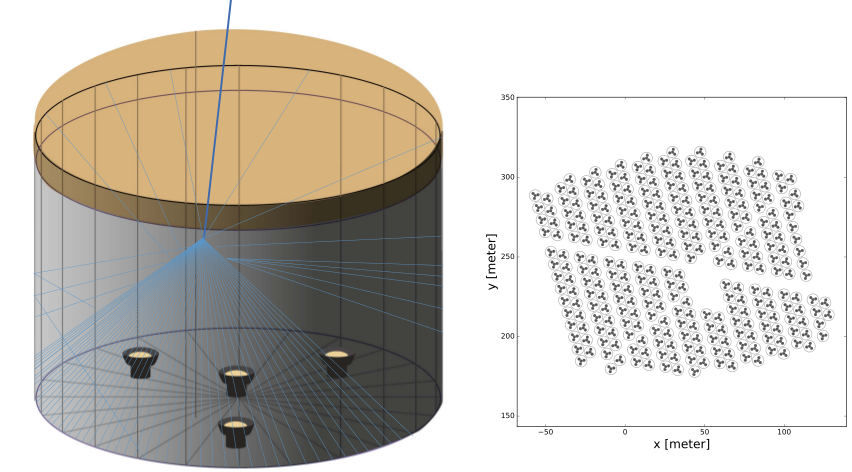
\includegraphics[scale = 0.3]{FIGURAS/TANQUE_HAWC.png}
		\caption{Lado izquierdo, esquema de un detector de agua Cherenkov. Lado derecho, esquema de distribución de los detectores en el observatorio HAWC \cite{Abeysekara}}.
		\label{TANQUE_HAWC}
	\end{figure}

	\subsection{Detectores Cherenkov}\label{DETECTORES_CHERENKOV}
		Los detectores Cherenkov de agua, o WCD por sus siglas en inglés Water Cherenkov Detector, han sido usados para la detección y construcción del espectro de CR's. Cada WCD tiene dimensiones de altura y diámetro variables dependiendo del observatorio; por ejemplo, Pierre Auger utiliza tanques de 1.55m de altura y 1.8m de diámetro. Un Tyvek reflectivo cubre internamente el tanque, el cual contiene agua purificada.
		
		\begin{figure}[h]
			\centering
			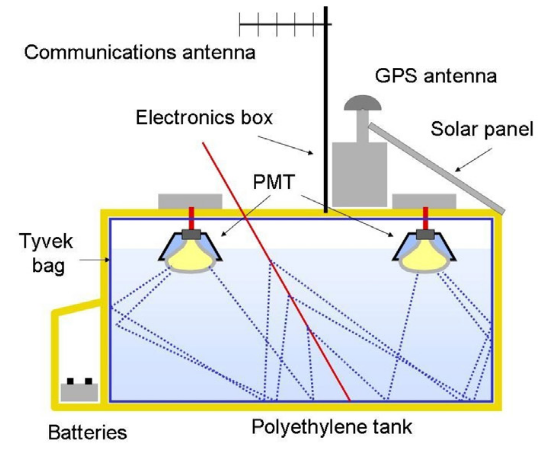
\includegraphics[scale = 0.5]{FIGURAS/TANQUE_CHERENKOV.png}
			\caption{Esquema de un WCD. Los fotones emitidos por las partículas cargadas al interacciones con el medio son detectados por los PMT \cite{LU2020163678}.}
			\label{TANQUE_CHERENKOV}
		\end{figure}
	
		Dentro del tanque además, se utilizan tubos fotomultiplicadores, o PMT's por sus siglas en inglés Photomultiplier Tubes, para la detección y amplificación de la señal de los fotones Cherenkov. Un amplificador es conectado en el último dínodo del PMT para una amplificación adicional a la señal. Los tanques pueden ser energéticamente autosuficientes usando paneles solares y baterias, además se puede manejar una sincronización temporal con la oficina central usando un GPS (Global Position System). Además, los datos pueden ser almacenados y procesados usando un micro-controlador para posteriormente ser enviados a la oficina central \cite{LU2020163678}. Dicho esquema de los WCD's se presenta en la fig. \ref{TANQUE_CHERENKOV}.
	
	\chapter{Decaimiento del muón y espectro de Michel}\label{DEC_MUON_MICHEL}
\section{Decaimiento del muón}
	El muón, al igual que el electrón, se encuentra dentro del grupo de los leptones en el modelo estándar, ambos presentan características similares, tienen la misma carga y el mismo espín ($1/2$), pero la principal diferencia se encuentra en la masa, la masa del muón es aproximadamente 200 veces la masa del electrón y además es inestable, por consiguiente, el muón decae en un electrón y dos neutrinos,\\
	\begin{equation}
	\mu^{-} \rightarrow e^{-}+\Bar{\nu_{e}}+\nu_{\mu}
	\end{equation}
	con un tiempo de vida media de $\tau=(2.19698110\pm 0000022)\mu s$ \cite{Olive_2014}. Este decaimiento puede ser ilustrado mediante diagramas de Feynman como se muestra en la figura \ref{MUON_DECAY}.
	
	\begin{figure}[h]
		\centering
		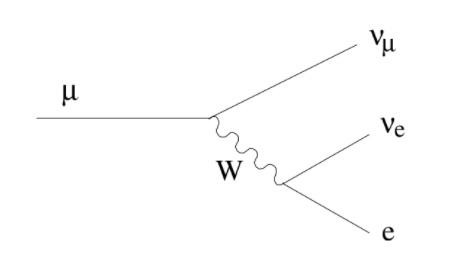
\includegraphics[scale = 0.65]{FIGURAS/MUON_DECAY.png}
		\caption{Proceso del decaimiento del muón.}
		\label{MUON_DECAY}
	\end{figure}

	Sin embargo en la naturaleza, y debido a las cascadas producidas por los rayos cósmicos primarios (ver sec.\ref{EAS}) se producen partículas muonicas positivas y negativas, lo que tiene un efecto al momento de medir su tiempo de decaimiento dentro de los tanques Cherenkov de agua. Los muones negativos, al momento de interaccionar con el medio (agua) va a sufrir lo que se conoce como captura muonica, lo que conlleva a que su tiempo de decaimiento sea menor, lo que no sucede con los muones positivos. Por ende, en los experimentos donde se desea obtener el $\tau$, éste va ser un promedio de ambos tiempo de vida media; entonces podemos decir que si nosotros logramos medir $\tau=2.196 \mu s$ nos indicaría que hay más presencia de muones positivos \cite{Holmlid}.
	
	El electrón que resulta del decaimiento del muón es conocido como electrón de Michel \cite{michel}. El análisis de la distribución de energía de estos electrones de Michel representa un punto de calibración en nuestros detectores Cherenkov, de esta manera, obtenemos un monitoreo continuo del funcionamiento y hasta del nivel de agua de los mismos \cite{ZUO20181}.

\section{Espectro de Michel}\label{ESPECTRO_MICHEL}
	El proceso en el que un muón decae en un electrón y dos neutrinos se le conoce a menudo como decaimiento Michel \cite{RENGA2019100029}. Debido a su corta energía, en promedio de 37 MeV y máximo 53 MeV, los electrones del Michel depositan toda su energía dentro de un tanque, por lo que la energía depositada en el tanque es independiente del nivel de agua \cite{ZUO20181}. Obtener un espectro de Michel (distribución energética de los electrones de Michel) puro es complicado experimentalmente ya que es casi imposible eliminar la contribución de los rayos cósmicos de fondo en dicho rango de energía, los rayos cósmicos de fondo es la radiación de fondo en la superficie que logra entrar al tanque y ser detectado por los PMT. Por lo tanto, para la obtención del espectro de Michel se suele recurrir a la simulación, ver figura \ref{MICHEL_ESPECTRO_SIMULADO}.
	
	\begin{figure}[h]
		\centering
		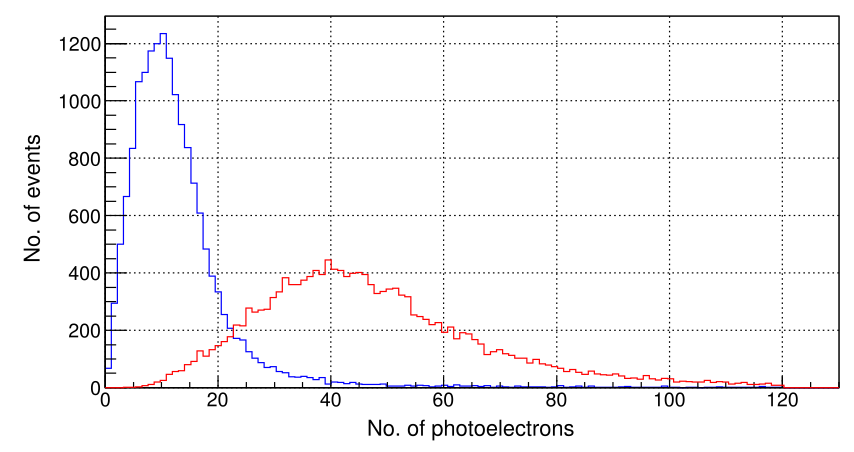
\includegraphics[scale = 0.45]{FIGURAS/ESPECTRO_MICHEL_SIMULADO.png}
		\caption{Distribución energética de los electrones de Michel (línea azul) y distribución energética de los muones frenados dentro del tanque (linea roja) \cite{ZUO20181}. Note que el número de fotoelectrones (eje X) es proporcional a la energía.}
		\label{MICHEL_ESPECTRO_SIMULADO}
	\end{figure}
	
	\chapter{Observatorios y colaboraciones que usan WCD's}\label{OBSERVATORIOS_COLABORACIONES}
\section{Observatorios}
	\subsection{LHAASO (The Large High Altitude Air Shower Observatory)}\label{LHAASO}
	El observatorio LHAASO se construirá en China, provincia de Sichuan, a una altura de 4400 m.s.n.m., el arreglo completo incluye alrededor de 1171 detectores de muones con el objetivo de estudiar y entender mejor las fuentes de los rayos cósmicos ultra-energéticos, por lo que su rango de energía en el cual se enfoca es desde los $10^{13}-10^{18} eV$. LHAASO tiene un area de detección de $40000 m^{2}$ donde de colocarán las unidades MD (muon detector). Dentro de los tanques (altura de 1,2 m y diámetro de 6,8 ) se coloca un material altamente reflectante y un tubo fotomultiplicador de 8 pulgadas \cite{ZUO20181}.
	
	\subsection{HAWC (High Altitude Water Cherenkov)}\label{HAWC}
	El observatorio de rayos gamma HAWC se encuentra situado en Sierra Negra, Mexico a aproximadamente 4100 msnm. HAWC es una colaboración internacional en la cual participan más de 30 investigadores de Mexico y EEUU con el objetivo de detectar rayos gamma con energía de entre 100 GeV y 100 TeV y con ello extender nuestro conocimiento de las fuentes cósmicas de los rayos gamma \cite{Bonilla}.
	
	\subsection{Pierre Auger}\label{PIERRE_AUGER}
	Construido en la provincia de Mendoza, Argentina, el Observatorio Pierre Auger es el observatorio más grande actualmente para medir rayos cósmicos de energía ultra alta con energías de hasta $10^{18} $eV. Este observatorio utiliza dos tipos de detectores: el primero es de superficie o detector Cherenkov de Agua (WCD), ver fig.~\ref{TANQUE_PIERRE_AUGER}, cuya finalidad es de reconstruir el desarrollo lateral de las lluvias por medio de la detección de partículas que llega al detector. El segundo son los telescopios de fluorescencia que son utilizados para el estudio de la longitud de desarrollo de las lluvias \cite{A.C.Cobos}.

	\begin{figure}[h]
		\centering
		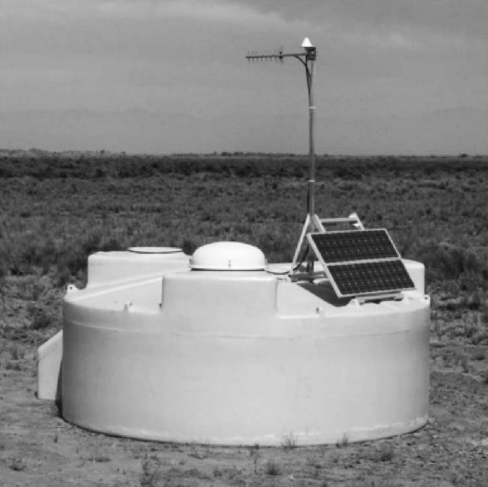
\includegraphics[scale=0.6]{FIGURAS/TANQUE_PIERRE_AUGER.PNG}
		\caption{Una estación de detacción instalada en el Observatorio Pierre Auger}
		\label{TANQUE_PIERRE_AUGER}
	\end{figure}

\section{Colaboraciones SWGO y LAGO}
	\subsection{Colaboración SWGO (Southern Wide-field Gamma-ray Observatory)}\label{SWGO}
	La detección de rayos gamma y CR han demostrado un importante potencial científico gracias a los observatorios de HAWC y LHAASO. Sin embargo, estos operan observando el hemisferio norte, por lo que la colaboración SWGO pretende ampliar ese campo de visión y mapeo del universo hacia el hemisferio sur, ver fig. \ref{MAPEO_SWGO}, construyendo observatorios que usen la tecnología de los WCD. El acceso al centro galáctico y el trabajo complementario con el observatorio CTA-Sur forman también parte de sus motivaciones para la construcción de un observatorio en el hemisferio sur \cite{schoorlemmer2019nextgeneration}. Una de las condiciones de SWGO para la construcción de un observatorio es que el lugar este situado a gran altitud, por lo que ciertas partes partes de la región Arequipa, Perú representan lugares prometedores para un futuro observatorio. Por otro lado SWGO tiene una red amplia de colaboradores alrededor del mundo, entre ellos se encuentra Perú, bajo la dirección y representación del Dr. José Bellido Cáceres, y la Universidad Nacional de San Agustín de Arequipa.
	
	\begin{figure}[h]
		\centering
		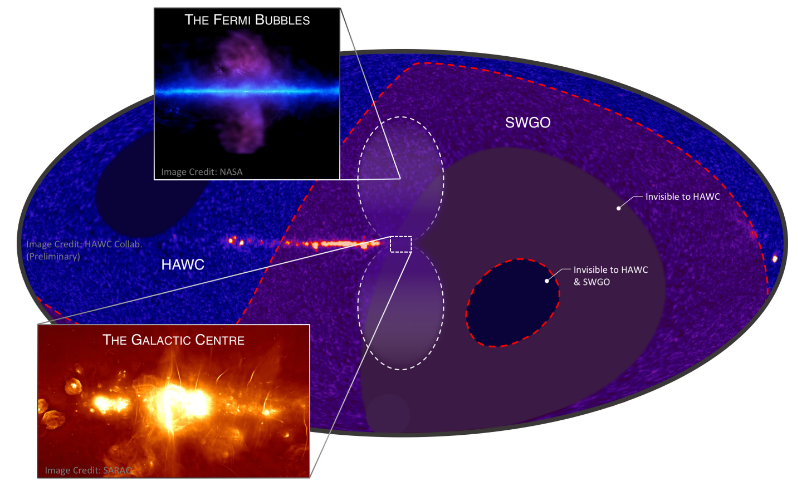
\includegraphics[scale = 0.45]{FIGURAS/MAPEO_SWGO.png}
		\caption{Mapeo que pretende realizar la colaboración SWGO (zona sombreada de rojo) mediante la construcción de un observatorio en el hemisferio sur \cite{schoorlemmer2019nextgeneration}.}
		\label{MAPEO_SWGO}
	\end{figure}
	
	\subsection{Colaboración LAGO (Latin American Giant Observatory)}\label{LAGO}
	La colaboración LAGO es un observatorio compuesto por una red de WCD's distribuidos por toda latino-américa, es decir, WCD's situados en diferentes lugares a diferentes altitudes, desde el nivel del mar hasta 5000 msnm. Los detectores de LAGO pueden contener de 1 a 40m$^3$ de agua purificada. Este observatorio esta diseñado para medir la evolución temporal del flujo de rayos cósmicos provinientes del espacio exterior evaluando tres aspectos: fenómenos de alta energía, clima espacial y radiación atmosférica a nivel del suelo. LAGO es entonces, una colaboración descentralizada que se expande desde el sur de México hasta la Patagonia gracias a la colaboración de más de 30 instituciones de 10 paises \cite{SIDELNIK2017173}. Para el desarrollo de la presente actividad se trabajó con datos compartidos por el proyecto LAGO, buscando los protocolos de calibración para estos detectores.
	
	
	
	\bibliographystyle{apalike}
	\bibliography{bibliografia.bib}
\end{document}
